\documentclass[a4paper]{article}

%% Language and font encodings
\usepackage[english]{babel}
\usepackage[utf8x]{inputenc}
\usepackage[T1]{fontenc}

%% Sets page size and margins
\usepackage[a4paper,top=3cm,bottom=2cm,left=3cm,right=3cm,marginparwidth=1.75cm]{geometry}

%% Useful packages
\usepackage{amsmath}
\usepackage{graphicx}
\graphicspath{ {images/} }

\usepackage[colorlinks=true, allcolors=blue]{hyperref}

\title{Assignment 3 - Software Design Specification and User Interface}
\author{ by Group 3 - Plant-Id \\* \\* Team Members: \\* Ethan Ahuja - ahujae \\* Ethan Patterson - patteret \\* James Barry - barryj \\* Evan Brass - brassev \\* Zachary Comito - comitoz \\* \\* Customers: \\* Ethan Ahuja - ahujae \\* Ethan Patterson - patteret }

\begin{document}
\maketitle
\pagebreak
`\tableofcontents
\pagebreak
\section{User Interface Prototypes}
\subsection{Home Screen}
\paragraph{Description:}Home screen will display 3 options to the user: 20 Questions, Photo-Id, and Help.
\begin{itemize}
\item 20 Questions: Takes user to decision to to identify users specimen.
\item Photo-Id: Takes user to a camera to identify the users specimen.
\item Help: Takes user to a help section of the application. 
\end{itemize}
\begin{center}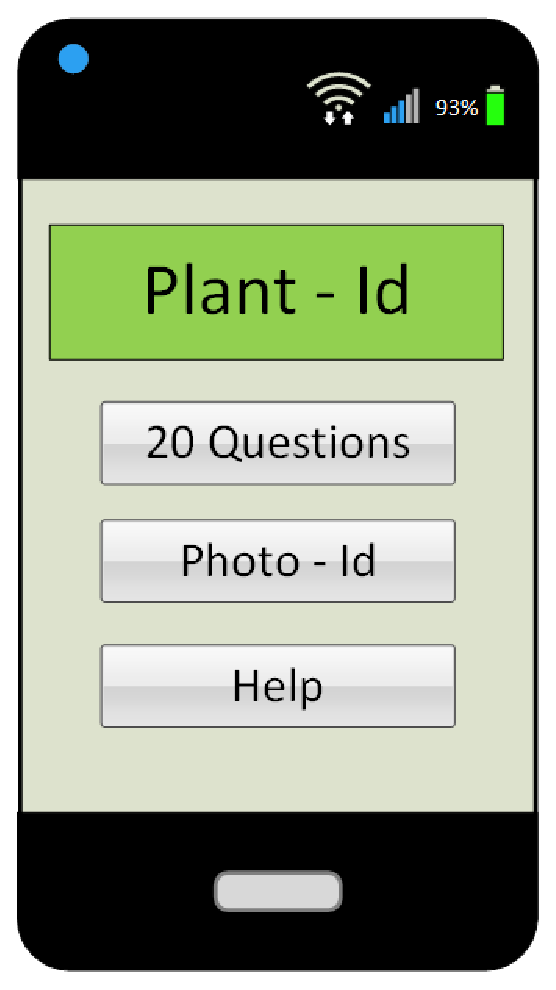
\includegraphics[scale=.8]{HomeScreen.eps}\end{center}
\pagebreak
\subsection{20 Questions}
\paragraph{Description:}
Example of use case one. Asks the user yes or no questions, or shows sets of images for the user to select. When done the user will be told the name of the specimen they are observing.
\paragraph{What you see:}
Bellow the user is presented with 4 images of leaf shapes. The user can select the closest matching leaf, or none of the above. In the top left corner of the phone screen is a \# symbol, this indicates what question the user is currently on.
\begin{center}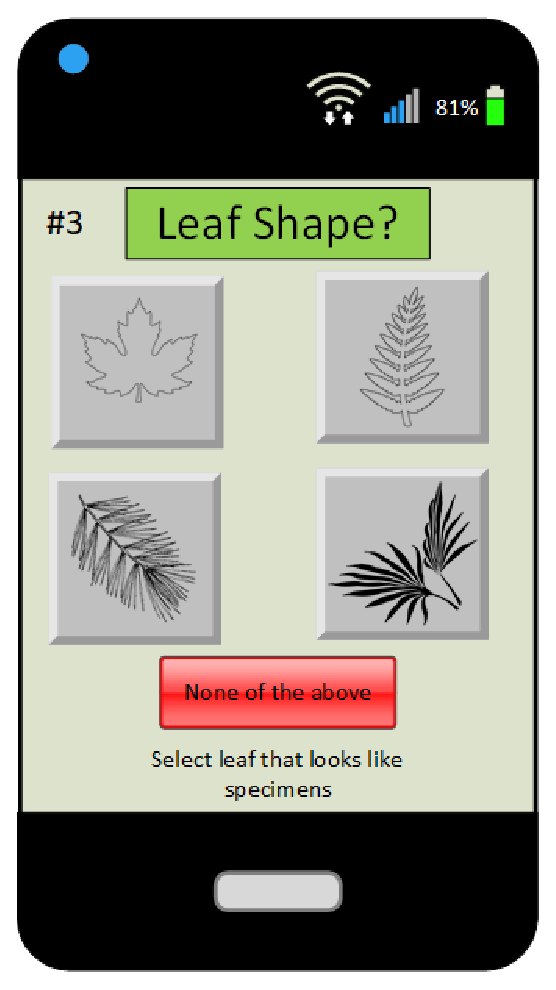
\includegraphics[scale=.8]{20Questions.eps}\end{center}
\pagebreak
\subsection{Photo-Id}
\paragraph{Description:}
Example of use case 3. The user takes multiple photos of the specimen, previously taken photo can be seen in the bottom right of the phone.
Once the user has taken a multiple photos, the neural network will this process these images and output the name of what it believes the specimen's name is.
\paragraph{What you see:}The camera interface for the application borrows its interface design from the default camera that comes on all android phones. This is to provide the user with a familiar, and comfortable, interface to interact with.
\begin{center}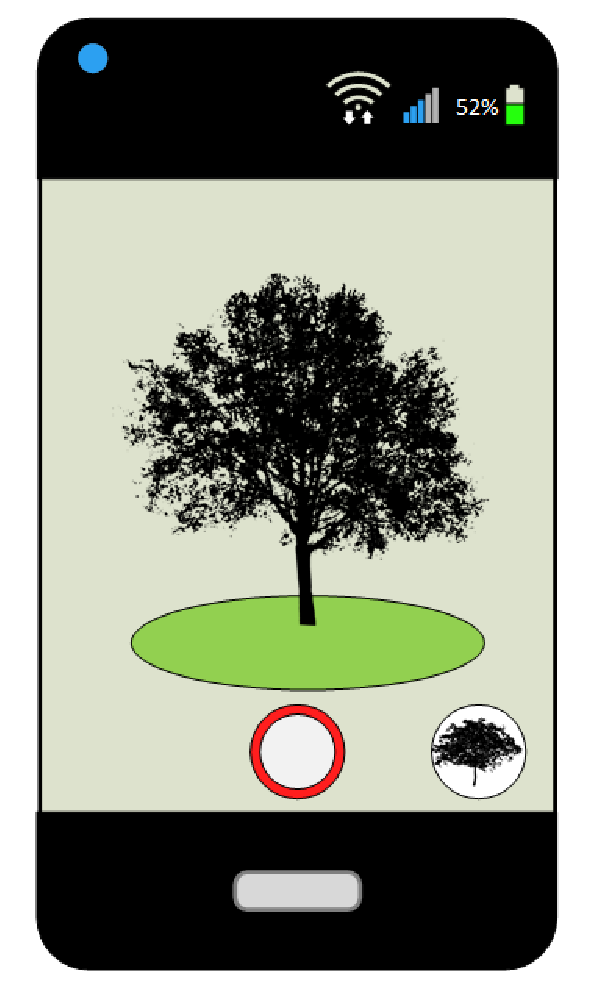
\includegraphics[scale=.8]{Photo-Id.eps}\end{center}
\pagebreak
\subsection{Program guess with error}
\paragraph{Description:}
This page shows what the final page after the 20 question page, or photo-Id page. In this example the user answered the questions randomly, resulting in an incorrect guess. This is the type of errors a user can expect to see:
\begin{itemize}
\item Guessing the answer to a question.
\item Plant might not be in data base.
\end{itemize}
These errors will not break our program, however it will cause the program to guess incorrectly. This certainty in a guess is displayed to a user with a percentage in certainty. If the user feels this is a mistake they can send us the bad data. A small text box will appear asking for what they believe the plant to be.
\paragraph{Plant mapping:} At the end of a guess a user has the option to send their GPS coordinates, when reconnected to a signal, So the application can map locations of plants found by users. This is optional. 
\begin{center}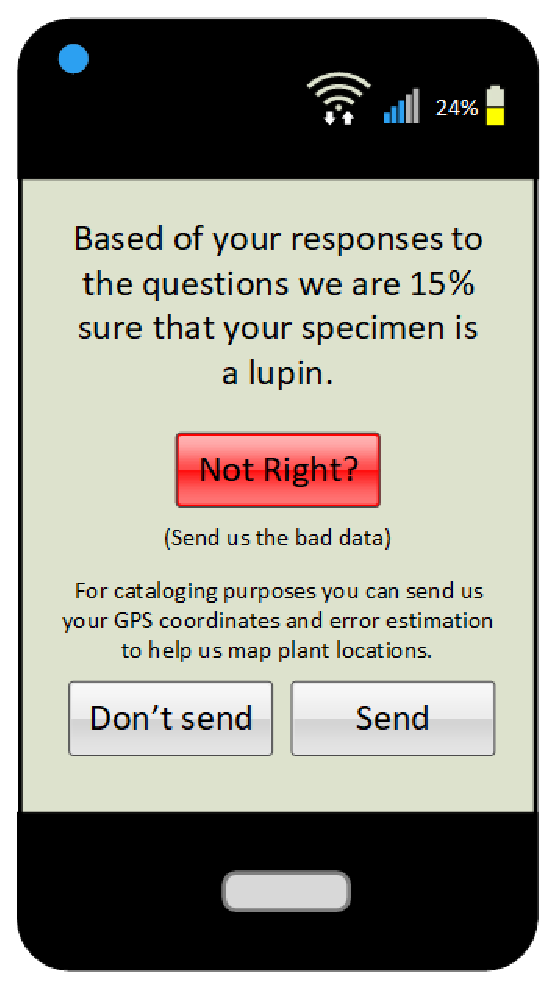
\includegraphics[scale=.8]{FinalPageWithError.eps}\end{center}
\pagebreak
\subsection{Help Screen}
\paragraph{Description:} The help screen provides three options to the user: Settings, How it Works, and a Contact Us option.
\begin{itemize}
\item Settings: Takes the user to application settings.
\item How it Works: Takes the user to a page explaining how the algorithms work.
\item Contact Us: Takes the user to a page that will allow them to send messages to the development team.
\end{itemize}
\begin{center}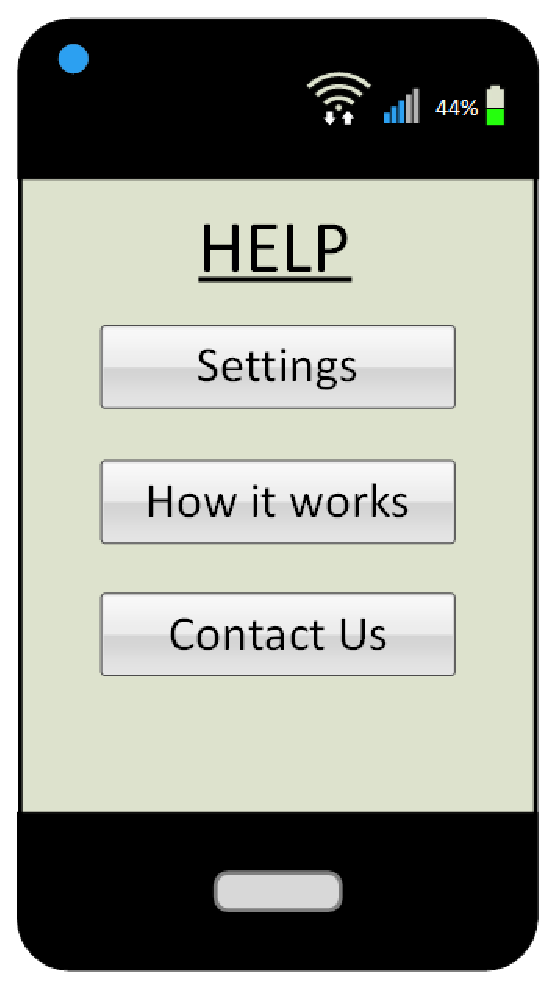
\includegraphics[scale=.8]{Help.eps}\end{center}
\pagebreak
\subsection{Settings}
\paragraph{Description:}
Example of use case 2. The Settings page gives the user control over some of the features of the application such as GPS tracking and auto updates.
\paragraph{What you see:} The user will be able to toggle radio buttons, possibly sliders, on or off to enable or disable application features.
\begin{center}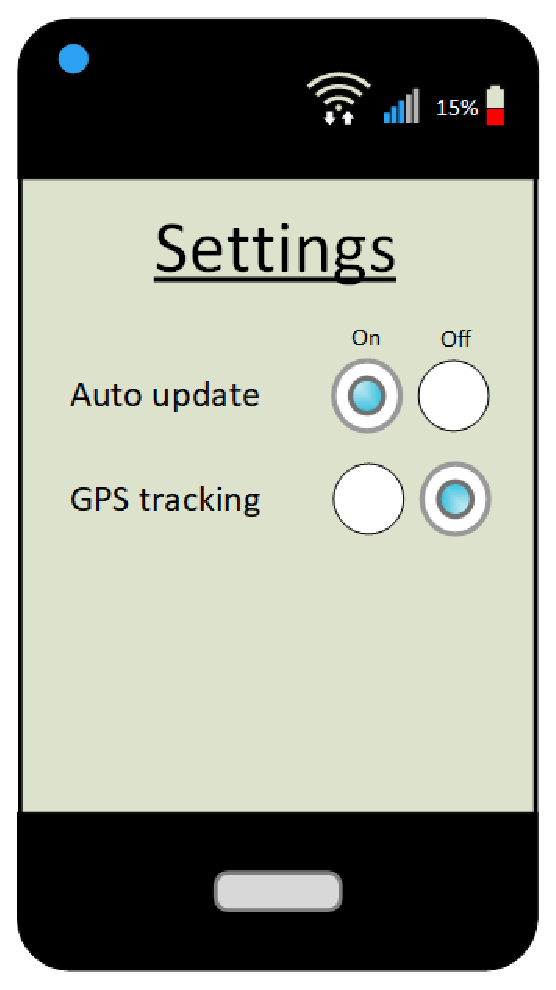
\includegraphics[scale=.8]{Settings.eps}\end{center}
\pagebreak
\subsection{How it Works}
\paragraph{Description:} The How it works page will give more information to the curious users on how the application is able to find an individual specimens name.
\begin{center}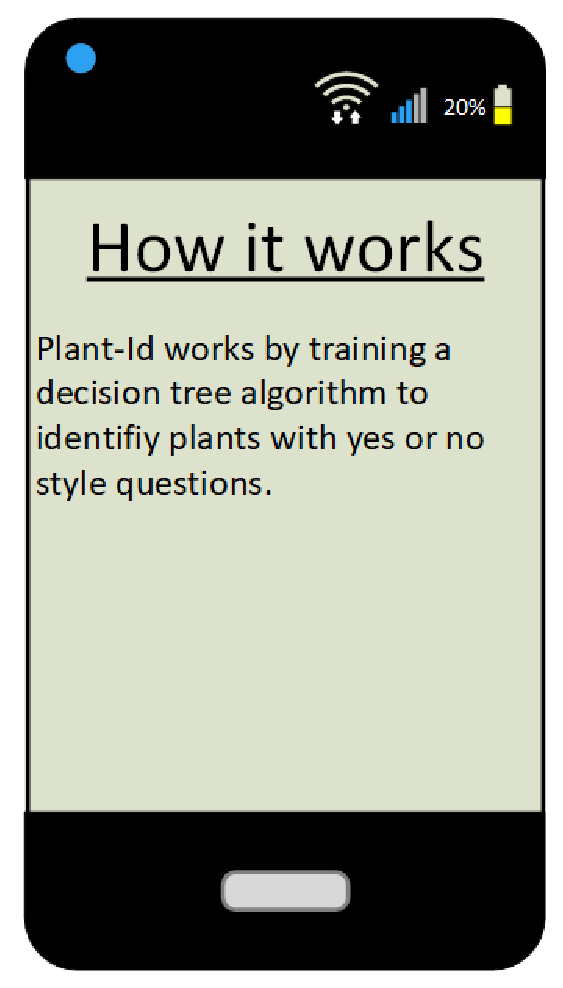
\includegraphics[scale=.8]{HowItWorks.eps}\end{center}
\pagebreak
\subsection{Contact Us}
\paragraph{Description:} The contact us page will allow the user to send messages to the development team. This will allow the team to receive vital feed back from the community using the application.
\paragraph{What you see:} Topic will be a key word to send the message with a tag. This will allow the developers to organize messages sent to them by topic.
\begin{center}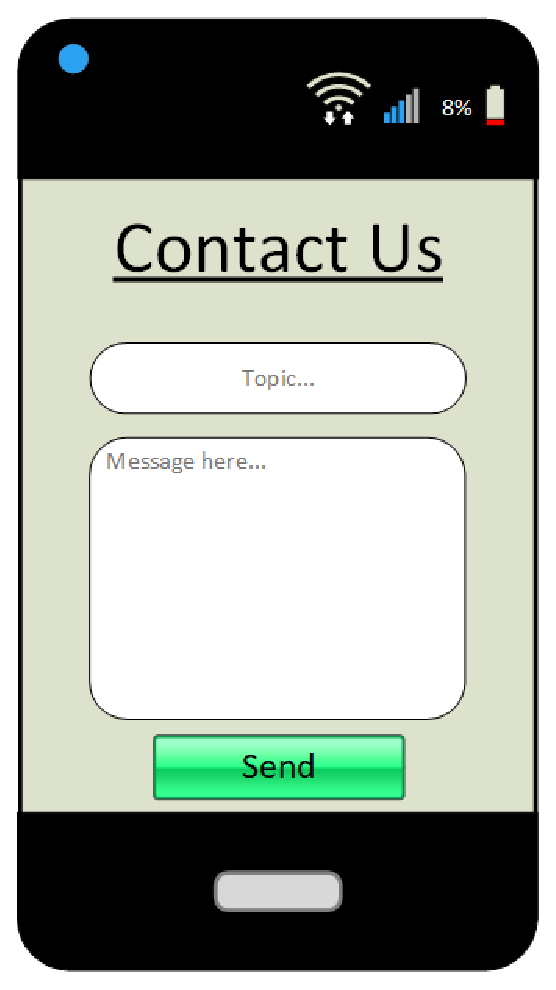
\includegraphics[scale=.8]{ContactUs.eps}\end{center}
\pagebreak
\section{Class Diagrams}
Our classes will be spread across three systems: An Android Java Application (No Kotlin actually), a server for training the decision tree, a webserver with a rest api that will mediate access to the database and support image upload for unrecognized plants.  The database is an SQL database with the following model (data types, like the length of the strings, may change):
\begin{center}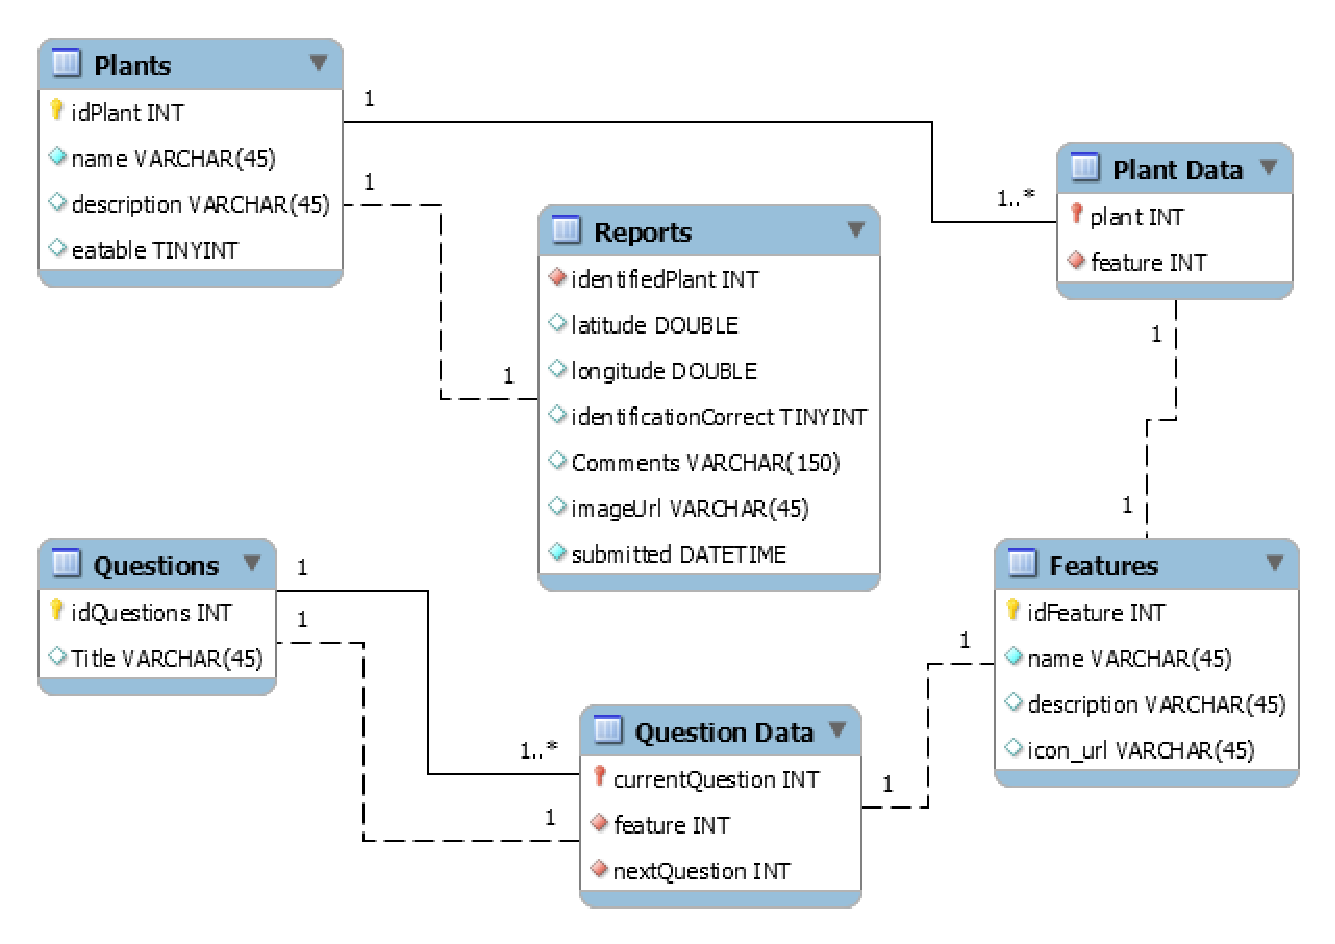
\includegraphics[scale=.6]{DatabaseDesign.eps}\end{center}
Each implementation (Android, training server, and REST server) will have their own classes that reflect this data and will expose methods for creation and deletion of these objects.  Our project is largely based on constructing a dataset so our classes don't need very many methods.  The real magic will be constructing the question sequence, and displaying it in a visually pleasing manner.
\pagebreak
\section{Sequence Diagrams}
\subsection{Question Based Identification}
This sequence diagram covers our first key use case, the 20 questions case. It explains the process of the app asking the user questions to help them identify a plant.
\begin{center}\includegraphics[scale=.8]{QuestionIdentification.eps}\end{center}
\pagebreak
\subsection{Image Based Identification}
This sequence diagram covers our third key use case, the Photo-Id case. It explains how the user can take multiple photos of a plant they want to identify and then have our neural network identify the plant for them.
\begin{center}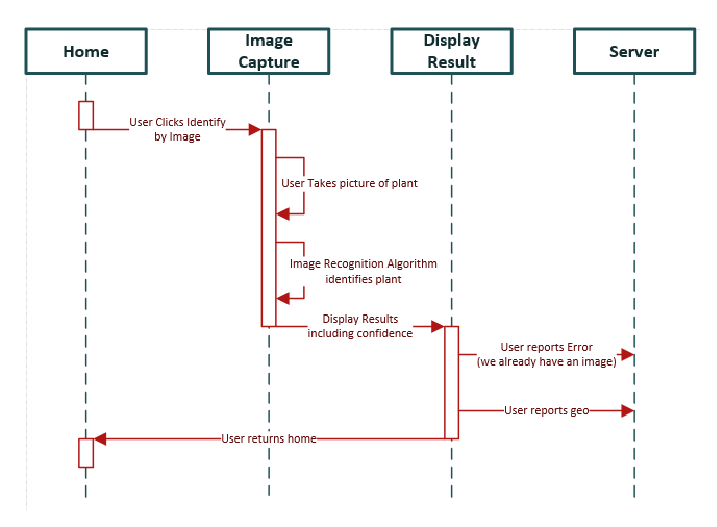
\includegraphics[scale=1.2]{ImageIdentification.eps}\end{center}
\pagebreak
\subsection{Botanist Report Review}
This sequence diagram describes the botanist report use case. It explains how a botanist can respond to reports of unidentified plants, or take a look at geotag information for discovered plants.
\begin{center}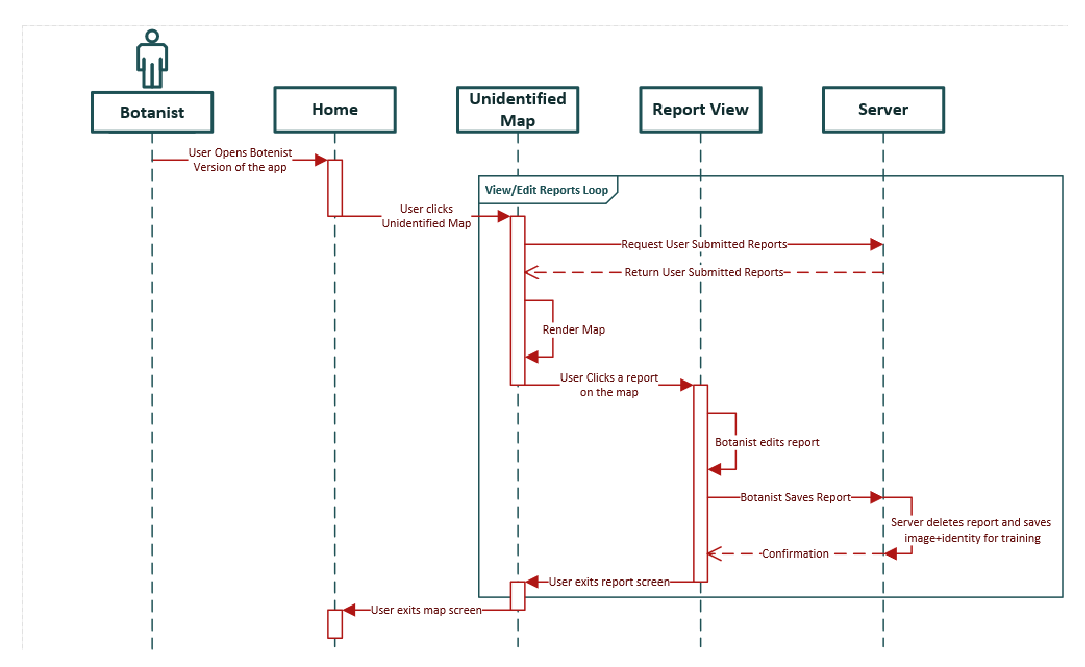
\includegraphics[scale=.8]{BotanistWorkflow.eps}\end{center}
\pagebreak
\section{Meeting Report}
\textbf{02/3/2018 (2:00pm - 6:00pm):} Johnson Hall - Room 219
\begin{itemize}
\item We created detailed diagrams of how our UI will be implemented. We Discussed critical features and how to tackle problems that may arise in the development process.
\item Next week we would like to implement an example decision tree in python and walk through the algorithm as a team to help the development team understand and ask questions about the ID3 algorithm.
\item Evan Brass and Ethan Ahuja created and documented the above Sequence Diagrams. Evan Brass created and documented the above Class Diagrams. Ethan Patterson created and documented the above User Interface Prototypes. James Barry worked remotely and assisted in writing and formating this document. James and Evan also met on Monday, February 5th, to finalize the document and clarify any vague or missing information. We were again unable to contact Zachary Comito.
\item Both customers, Ethan Patterson and Ethan Ahuja, were able to attend this weeks meeting.
\end{itemize}
\newpage %Move references to the next page..
\begin{thebibliography}{9}
\bibitem{latexcompanion} 
\url{http://www.saedsayad.com/decision_tree.htm}
Dr. Saed Sayad, Reading, www, 2010-2018.
\bibitem{einstein} 
Victor Lavrenko.
\url{https://www.youtube.com/watch?v=eKD5gxPPeY0&list=PLBv09BD7ez_4temBw7vLA19p3tdQH6FYO}
\textit{School of Informatics} 
[\textit{Decision Trees}]. 
Victor Lavrenko and Nigel Goddard, January 19, 2014.
\bibitem{3blueOneBrown}
[\textit{Neural Network}]
YouTube, YouTube, 5 Oct. 2017, \url{www.youtube.com/watch?v=aircAruvnKk&list=PLZHQObOWTQDNU6R1_67000Dx_ZCJB-3pi}
\bibitem{Nielsen, Michael A}
[\textit{Neural Network}
Nielsen, Michael A. “Neural Networks and Deep Learning.” Neural networks and deep learning, Determination Press, 1 Jan. 1970,\url{ neuralnetworksanddeeplearning.com/}.
\end{thebibliography}
\end{document}